% Created by tikzDevice version 0.12.6 on 2025-04-16 10:39:48
% !TEX encoding = UTF-8 Unicode
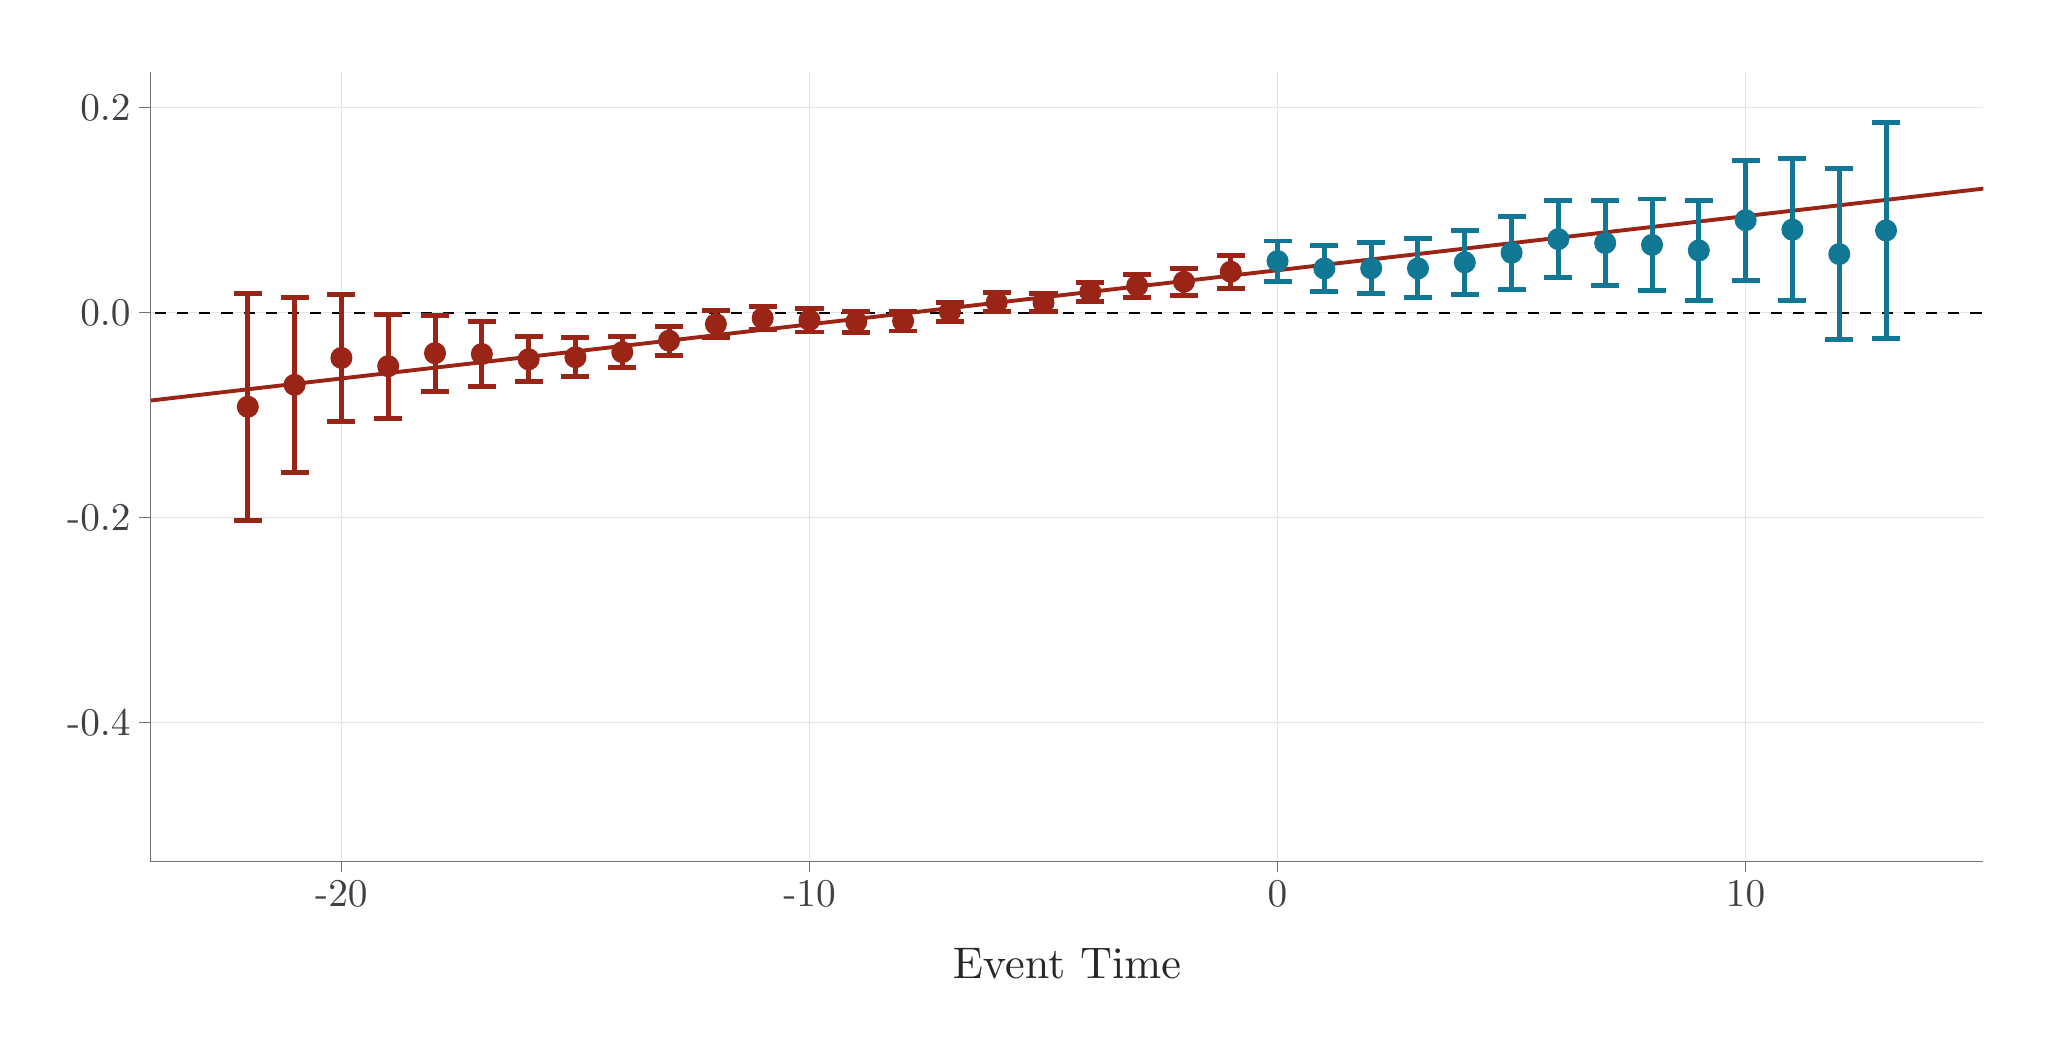
\begin{tikzpicture}[x=1pt,y=1pt]
\definecolor{fillColor}{RGB}{255,255,255}
\path[use as bounding box,fill=fillColor] (0,0) rectangle (722.70,361.35);
\begin{scope}
\path[clip] (  0.00,  0.00) rectangle (722.70,361.35);
\definecolor{drawColor}{RGB}{255,255,255}

\path[draw=drawColor,line width= 0.8pt,line join=round,line cap=round,fill=fillColor] (  0.00,  0.00) rectangle (722.70,361.35);
\end{scope}
\begin{scope}
\path[clip] ( 44.36, 60.16) rectangle (706.70,345.35);
\definecolor{drawColor}{RGB}{255,255,255}
\definecolor{fillColor}{RGB}{255,255,255}

\path[draw=drawColor,line width= 0.8pt,line join=round,line cap=round,fill=fillColor] ( 44.36, 60.16) rectangle (706.70,345.35);
\definecolor{drawColor}{RGB}{228,228,231}

\path[draw=drawColor,line width= 0.4pt,line join=round] ( 44.36,110.16) --
	(706.70,110.16);

\path[draw=drawColor,line width= 0.4pt,line join=round] ( 44.36,184.23) --
	(706.70,184.23);

\path[draw=drawColor,line width= 0.4pt,line join=round] ( 44.36,258.31) --
	(706.70,258.31);

\path[draw=drawColor,line width= 0.4pt,line join=round] ( 44.36,332.39) --
	(706.70,332.39);

\path[draw=drawColor,line width= 0.4pt,line join=round] (113.37, 60.16) --
	(113.37,345.35);

\path[draw=drawColor,line width= 0.4pt,line join=round] (282.50, 60.16) --
	(282.50,345.35);

\path[draw=drawColor,line width= 0.4pt,line join=round] (451.64, 60.16) --
	(451.64,345.35);

\path[draw=drawColor,line width= 0.4pt,line join=round] (620.78, 60.16) --
	(620.78,345.35);
\definecolor{drawColor}{RGB}{0,0,0}

\path[draw=drawColor,line width= 0.9pt,dash pattern=on 4pt off 4pt ,line join=round] (-617.98,258.31) -- (1369.04,258.31);
\definecolor{drawColor}{RGB}{154,36,21}

\path[draw=drawColor,line width= 1.4pt,line join=round] (-617.98,150.02) -- (1369.04,379.77);
\definecolor{fillColor}{RGB}{154,36,21}

\path[draw=drawColor,line width= 0.5pt,line join=round,line cap=round,fill=fillColor] ( 79.54,224.36) circle (  3.73);

\path[draw=drawColor,line width= 0.5pt,line join=round,line cap=round,fill=fillColor] ( 96.45,232.28) circle (  3.73);

\path[draw=drawColor,line width= 0.5pt,line join=round,line cap=round,fill=fillColor] (113.37,242.01) circle (  3.73);

\path[draw=drawColor,line width= 0.5pt,line join=round,line cap=round,fill=fillColor] (130.28,239.02) circle (  3.73);

\path[draw=drawColor,line width= 0.5pt,line join=round,line cap=round,fill=fillColor] (147.19,243.72) circle (  3.73);

\path[draw=drawColor,line width= 0.5pt,line join=round,line cap=round,fill=fillColor] (164.11,243.42) circle (  3.73);

\path[draw=drawColor,line width= 0.5pt,line join=round,line cap=round,fill=fillColor] (181.02,241.51) circle (  3.73);

\path[draw=drawColor,line width= 0.5pt,line join=round,line cap=round,fill=fillColor] (197.94,242.27) circle (  3.73);

\path[draw=drawColor,line width= 0.5pt,line join=round,line cap=round,fill=fillColor] (214.85,244.11) circle (  3.73);

\path[draw=drawColor,line width= 0.5pt,line join=round,line cap=round,fill=fillColor] (231.76,248.25) circle (  3.73);

\path[draw=drawColor,line width= 0.5pt,line join=round,line cap=round,fill=fillColor] (248.68,254.22) circle (  3.73);

\path[draw=drawColor,line width= 0.5pt,line join=round,line cap=round,fill=fillColor] (265.59,256.38) circle (  3.73);

\path[draw=drawColor,line width= 0.5pt,line join=round,line cap=round,fill=fillColor] (282.50,255.68) circle (  3.73);

\path[draw=drawColor,line width= 0.5pt,line join=round,line cap=round,fill=fillColor] (299.42,255.08) circle (  3.73);

\path[draw=drawColor,line width= 0.5pt,line join=round,line cap=round,fill=fillColor] (316.33,255.34) circle (  3.73);

\path[draw=drawColor,line width= 0.5pt,line join=round,line cap=round,fill=fillColor] (333.25,258.73) circle (  3.73);

\path[draw=drawColor,line width= 0.5pt,line join=round,line cap=round,fill=fillColor] (350.16,262.11) circle (  3.73);

\path[draw=drawColor,line width= 0.5pt,line join=round,line cap=round,fill=fillColor] (367.07,262.01) circle (  3.73);

\path[draw=drawColor,line width= 0.5pt,line join=round,line cap=round,fill=fillColor] (383.99,265.80) circle (  3.73);

\path[draw=drawColor,line width= 0.5pt,line join=round,line cap=round,fill=fillColor] (400.90,268.07) circle (  3.73);

\path[draw=drawColor,line width= 0.5pt,line join=round,line cap=round,fill=fillColor] (417.81,269.53) circle (  3.73);

\path[draw=drawColor,line width= 0.5pt,line join=round,line cap=round,fill=fillColor] (434.73,273.16) circle (  3.73);
\definecolor{drawColor}{RGB}{16,120,149}
\definecolor{fillColor}{RGB}{16,120,149}

\path[draw=drawColor,line width= 0.5pt,line join=round,line cap=round,fill=fillColor] (451.64,277.01) circle (  3.73);

\path[draw=drawColor,line width= 0.5pt,line join=round,line cap=round,fill=fillColor] (468.56,274.33) circle (  3.73);

\path[draw=drawColor,line width= 0.5pt,line join=round,line cap=round,fill=fillColor] (485.47,274.41) circle (  3.73);

\path[draw=drawColor,line width= 0.5pt,line join=round,line cap=round,fill=fillColor] (502.38,274.36) circle (  3.73);

\path[draw=drawColor,line width= 0.5pt,line join=round,line cap=round,fill=fillColor] (519.30,276.54) circle (  3.73);

\path[draw=drawColor,line width= 0.5pt,line join=round,line cap=round,fill=fillColor] (536.21,280.02) circle (  3.73);

\path[draw=drawColor,line width= 0.5pt,line join=round,line cap=round,fill=fillColor] (553.12,284.94) circle (  3.73);

\path[draw=drawColor,line width= 0.5pt,line join=round,line cap=round,fill=fillColor] (570.04,283.54) circle (  3.73);

\path[draw=drawColor,line width= 0.5pt,line join=round,line cap=round,fill=fillColor] (586.95,282.85) circle (  3.73);

\path[draw=drawColor,line width= 0.5pt,line join=round,line cap=round,fill=fillColor] (603.86,280.84) circle (  3.73);

\path[draw=drawColor,line width= 0.5pt,line join=round,line cap=round,fill=fillColor] (620.78,291.79) circle (  3.73);

\path[draw=drawColor,line width= 0.5pt,line join=round,line cap=round,fill=fillColor] (637.69,288.37) circle (  3.73);

\path[draw=drawColor,line width= 0.5pt,line join=round,line cap=round,fill=fillColor] (654.61,279.54) circle (  3.73);

\path[draw=drawColor,line width= 0.5pt,line join=round,line cap=round,fill=fillColor] (671.52,288.07) circle (  3.73);
\definecolor{drawColor}{RGB}{154,36,21}

\path[draw=drawColor,line width= 1.8pt,line join=round] ( 74.47,265.42) --
	( 84.61,265.42);

\path[draw=drawColor,line width= 1.8pt,line join=round] ( 79.54,265.42) --
	( 79.54,183.31);

\path[draw=drawColor,line width= 1.8pt,line join=round] ( 74.47,183.31) --
	( 84.61,183.31);

\path[draw=drawColor,line width= 1.8pt,line join=round] ( 91.38,263.81) --
	(101.53,263.81);

\path[draw=drawColor,line width= 1.8pt,line join=round] ( 96.45,263.81) --
	( 96.45,200.75);

\path[draw=drawColor,line width= 1.8pt,line join=round] ( 91.38,200.75) --
	(101.53,200.75);

\path[draw=drawColor,line width= 1.8pt,line join=round] (108.29,264.98) --
	(118.44,264.98);

\path[draw=drawColor,line width= 1.8pt,line join=round] (113.37,264.98) --
	(113.37,219.04);

\path[draw=drawColor,line width= 1.8pt,line join=round] (108.29,219.04) --
	(118.44,219.04);

\path[draw=drawColor,line width= 1.8pt,line join=round] (125.21,257.79) --
	(135.36,257.79);

\path[draw=drawColor,line width= 1.8pt,line join=round] (130.28,257.79) --
	(130.28,220.26);

\path[draw=drawColor,line width= 1.8pt,line join=round] (125.21,220.26) --
	(135.36,220.26);

\path[draw=drawColor,line width= 1.8pt,line join=round] (142.12,257.49) --
	(152.27,257.49);

\path[draw=drawColor,line width= 1.8pt,line join=round] (147.19,257.49) --
	(147.19,229.94);

\path[draw=drawColor,line width= 1.8pt,line join=round] (142.12,229.94) --
	(152.27,229.94);

\path[draw=drawColor,line width= 1.8pt,line join=round] (159.03,255.18) --
	(169.18,255.18);

\path[draw=drawColor,line width= 1.8pt,line join=round] (164.11,255.18) --
	(164.11,231.67);

\path[draw=drawColor,line width= 1.8pt,line join=round] (159.03,231.67) --
	(169.18,231.67);

\path[draw=drawColor,line width= 1.8pt,line join=round] (175.95,249.69) --
	(186.10,249.69);

\path[draw=drawColor,line width= 1.8pt,line join=round] (181.02,249.69) --
	(181.02,233.32);

\path[draw=drawColor,line width= 1.8pt,line join=round] (175.95,233.32) --
	(186.10,233.32);

\path[draw=drawColor,line width= 1.8pt,line join=round] (192.86,249.23) --
	(203.01,249.23);

\path[draw=drawColor,line width= 1.8pt,line join=round] (197.94,249.23) --
	(197.94,235.32);

\path[draw=drawColor,line width= 1.8pt,line join=round] (192.86,235.32) --
	(203.01,235.32);

\path[draw=drawColor,line width= 1.8pt,line join=round] (209.78,249.80) --
	(219.92,249.80);

\path[draw=drawColor,line width= 1.8pt,line join=round] (214.85,249.80) --
	(214.85,238.41);

\path[draw=drawColor,line width= 1.8pt,line join=round] (209.78,238.41) --
	(219.92,238.41);

\path[draw=drawColor,line width= 1.8pt,line join=round] (226.69,253.50) --
	(236.84,253.50);

\path[draw=drawColor,line width= 1.8pt,line join=round] (231.76,253.50) --
	(231.76,242.99);

\path[draw=drawColor,line width= 1.8pt,line join=round] (226.69,242.99) --
	(236.84,242.99);

\path[draw=drawColor,line width= 1.8pt,line join=round] (243.60,259.00) --
	(253.75,259.00);

\path[draw=drawColor,line width= 1.8pt,line join=round] (248.68,259.00) --
	(248.68,249.44);

\path[draw=drawColor,line width= 1.8pt,line join=round] (243.60,249.44) --
	(253.75,249.44);

\path[draw=drawColor,line width= 1.8pt,line join=round] (260.52,260.58) --
	(270.66,260.58);

\path[draw=drawColor,line width= 1.8pt,line join=round] (265.59,260.58) --
	(265.59,252.18);

\path[draw=drawColor,line width= 1.8pt,line join=round] (260.52,252.18) --
	(270.66,252.18);

\path[draw=drawColor,line width= 1.8pt,line join=round] (277.43,259.97) --
	(287.58,259.97);

\path[draw=drawColor,line width= 1.8pt,line join=round] (282.50,259.97) --
	(282.50,251.38);

\path[draw=drawColor,line width= 1.8pt,line join=round] (277.43,251.38) --
	(287.58,251.38);

\path[draw=drawColor,line width= 1.8pt,line join=round] (294.34,258.94) --
	(304.49,258.94);

\path[draw=drawColor,line width= 1.8pt,line join=round] (299.42,258.94) --
	(299.42,251.21);

\path[draw=drawColor,line width= 1.8pt,line join=round] (294.34,251.21) --
	(304.49,251.21);

\path[draw=drawColor,line width= 1.8pt,line join=round] (311.26,258.94) --
	(321.41,258.94);

\path[draw=drawColor,line width= 1.8pt,line join=round] (316.33,258.94) --
	(316.33,251.74);

\path[draw=drawColor,line width= 1.8pt,line join=round] (311.26,251.74) --
	(321.41,251.74);

\path[draw=drawColor,line width= 1.8pt,line join=round] (328.17,262.20) --
	(338.32,262.20);

\path[draw=drawColor,line width= 1.8pt,line join=round] (333.25,262.20) --
	(333.25,255.27);

\path[draw=drawColor,line width= 1.8pt,line join=round] (328.17,255.27) --
	(338.32,255.27);

\path[draw=drawColor,line width= 1.8pt,line join=round] (345.08,265.51) --
	(355.23,265.51);

\path[draw=drawColor,line width= 1.8pt,line join=round] (350.16,265.51) --
	(350.16,258.71);

\path[draw=drawColor,line width= 1.8pt,line join=round] (345.08,258.71) --
	(355.23,258.71);

\path[draw=drawColor,line width= 1.8pt,line join=round] (362.00,265.37) --
	(372.15,265.37);

\path[draw=drawColor,line width= 1.8pt,line join=round] (367.07,265.37) --
	(367.07,258.66);

\path[draw=drawColor,line width= 1.8pt,line join=round] (362.00,258.66) --
	(372.15,258.66);

\path[draw=drawColor,line width= 1.8pt,line join=round] (378.91,269.36) --
	(389.06,269.36);

\path[draw=drawColor,line width= 1.8pt,line join=round] (383.99,269.36) --
	(383.99,262.24);

\path[draw=drawColor,line width= 1.8pt,line join=round] (378.91,262.24) --
	(389.06,262.24);

\path[draw=drawColor,line width= 1.8pt,line join=round] (395.83,272.17) --
	(405.97,272.17);

\path[draw=drawColor,line width= 1.8pt,line join=round] (400.90,272.17) --
	(400.90,263.98);

\path[draw=drawColor,line width= 1.8pt,line join=round] (395.83,263.98) --
	(405.97,263.98);

\path[draw=drawColor,line width= 1.8pt,line join=round] (412.74,274.39) --
	(422.89,274.39);

\path[draw=drawColor,line width= 1.8pt,line join=round] (417.81,274.39) --
	(417.81,264.67);

\path[draw=drawColor,line width= 1.8pt,line join=round] (412.74,264.67) --
	(422.89,264.67);

\path[draw=drawColor,line width= 1.8pt,line join=round] (429.65,279.15) --
	(439.80,279.15);

\path[draw=drawColor,line width= 1.8pt,line join=round] (434.73,279.15) --
	(434.73,267.17);

\path[draw=drawColor,line width= 1.8pt,line join=round] (429.65,267.17) --
	(439.80,267.17);
\definecolor{drawColor}{RGB}{16,120,149}

\path[draw=drawColor,line width= 1.8pt,line join=round] (446.57,284.26) --
	(456.72,284.26);

\path[draw=drawColor,line width= 1.8pt,line join=round] (451.64,284.26) --
	(451.64,269.77);

\path[draw=drawColor,line width= 1.8pt,line join=round] (446.57,269.77) --
	(456.72,269.77);

\path[draw=drawColor,line width= 1.8pt,line join=round] (463.48,282.51) --
	(473.63,282.51);

\path[draw=drawColor,line width= 1.8pt,line join=round] (468.56,282.51) --
	(468.56,266.16);

\path[draw=drawColor,line width= 1.8pt,line join=round] (463.48,266.16) --
	(473.63,266.16);

\path[draw=drawColor,line width= 1.8pt,line join=round] (480.39,283.68) --
	(490.54,283.68);

\path[draw=drawColor,line width= 1.8pt,line join=round] (485.47,283.68) --
	(485.47,265.15);

\path[draw=drawColor,line width= 1.8pt,line join=round] (480.39,265.15) --
	(490.54,265.15);

\path[draw=drawColor,line width= 1.8pt,line join=round] (497.31,285.05) --
	(507.46,285.05);

\path[draw=drawColor,line width= 1.8pt,line join=round] (502.38,285.05) --
	(502.38,263.68);

\path[draw=drawColor,line width= 1.8pt,line join=round] (497.31,263.68) --
	(507.46,263.68);

\path[draw=drawColor,line width= 1.8pt,line join=round] (514.22,288.17) --
	(524.37,288.17);

\path[draw=drawColor,line width= 1.8pt,line join=round] (519.30,288.17) --
	(519.30,264.92);

\path[draw=drawColor,line width= 1.8pt,line join=round] (514.22,264.92) --
	(524.37,264.92);

\path[draw=drawColor,line width= 1.8pt,line join=round] (531.14,293.16) --
	(541.28,293.16);

\path[draw=drawColor,line width= 1.8pt,line join=round] (536.21,293.16) --
	(536.21,266.87);

\path[draw=drawColor,line width= 1.8pt,line join=round] (531.14,266.87) --
	(541.28,266.87);

\path[draw=drawColor,line width= 1.8pt,line join=round] (548.05,298.89) --
	(558.20,298.89);

\path[draw=drawColor,line width= 1.8pt,line join=round] (553.12,298.89) --
	(553.12,270.99);

\path[draw=drawColor,line width= 1.8pt,line join=round] (548.05,270.99) --
	(558.20,270.99);

\path[draw=drawColor,line width= 1.8pt,line join=round] (564.96,298.94) --
	(575.11,298.94);

\path[draw=drawColor,line width= 1.8pt,line join=round] (570.04,298.94) --
	(570.04,268.14);

\path[draw=drawColor,line width= 1.8pt,line join=round] (564.96,268.14) --
	(575.11,268.14);

\path[draw=drawColor,line width= 1.8pt,line join=round] (581.88,299.44) --
	(592.03,299.44);

\path[draw=drawColor,line width= 1.8pt,line join=round] (586.95,299.44) --
	(586.95,266.26);

\path[draw=drawColor,line width= 1.8pt,line join=round] (581.88,266.26) --
	(592.03,266.26);

\path[draw=drawColor,line width= 1.8pt,line join=round] (598.79,298.93) --
	(608.94,298.93);

\path[draw=drawColor,line width= 1.8pt,line join=round] (603.86,298.93) --
	(603.86,262.75);

\path[draw=drawColor,line width= 1.8pt,line join=round] (598.79,262.75) --
	(608.94,262.75);

\path[draw=drawColor,line width= 1.8pt,line join=round] (615.70,313.46) --
	(625.85,313.46);

\path[draw=drawColor,line width= 1.8pt,line join=round] (620.78,313.46) --
	(620.78,270.11);

\path[draw=drawColor,line width= 1.8pt,line join=round] (615.70,270.11) --
	(625.85,270.11);

\path[draw=drawColor,line width= 1.8pt,line join=round] (632.62,314.13) --
	(642.77,314.13);

\path[draw=drawColor,line width= 1.8pt,line join=round] (637.69,314.13) --
	(637.69,262.62);

\path[draw=drawColor,line width= 1.8pt,line join=round] (632.62,262.62) --
	(642.77,262.62);

\path[draw=drawColor,line width= 1.8pt,line join=round] (649.53,310.31) --
	(659.68,310.31);

\path[draw=drawColor,line width= 1.8pt,line join=round] (654.61,310.31) --
	(654.61,248.77);

\path[draw=drawColor,line width= 1.8pt,line join=round] (649.53,248.77) --
	(659.68,248.77);

\path[draw=drawColor,line width= 1.8pt,line join=round] (666.45,326.96) --
	(676.59,326.96);

\path[draw=drawColor,line width= 1.8pt,line join=round] (671.52,326.96) --
	(671.52,249.18);

\path[draw=drawColor,line width= 1.8pt,line join=round] (666.45,249.18) --
	(676.59,249.18);
\end{scope}
\begin{scope}
\path[clip] (  0.00,  0.00) rectangle (722.70,361.35);
\definecolor{drawColor}{RGB}{113,113,122}

\path[draw=drawColor,line width= 0.3pt,line join=round] ( 44.36, 60.16) --
	( 44.36,345.35);
\end{scope}
\begin{scope}
\path[clip] (  0.00,  0.00) rectangle (722.70,361.35);
\definecolor{drawColor}{RGB}{63,63,70}

\node[text=drawColor,anchor=base east,inner sep=0pt, outer sep=0pt, scale=  1.42] at ( 37.16,105.49) {-0.4};

\node[text=drawColor,anchor=base east,inner sep=0pt, outer sep=0pt, scale=  1.42] at ( 37.16,179.57) {-0.2};

\node[text=drawColor,anchor=base east,inner sep=0pt, outer sep=0pt, scale=  1.42] at ( 37.16,253.65) {0.0};

\node[text=drawColor,anchor=base east,inner sep=0pt, outer sep=0pt, scale=  1.42] at ( 37.16,327.72) {0.2};
\end{scope}
\begin{scope}
\path[clip] (  0.00,  0.00) rectangle (722.70,361.35);
\definecolor{drawColor}{RGB}{113,113,122}

\path[draw=drawColor,line width= 0.3pt,line join=round] ( 40.36,110.16) --
	( 44.36,110.16);

\path[draw=drawColor,line width= 0.3pt,line join=round] ( 40.36,184.23) --
	( 44.36,184.23);

\path[draw=drawColor,line width= 0.3pt,line join=round] ( 40.36,258.31) --
	( 44.36,258.31);

\path[draw=drawColor,line width= 0.3pt,line join=round] ( 40.36,332.39) --
	( 44.36,332.39);
\end{scope}
\begin{scope}
\path[clip] (  0.00,  0.00) rectangle (722.70,361.35);
\definecolor{drawColor}{RGB}{113,113,122}

\path[draw=drawColor,line width= 0.3pt,line join=round] ( 44.36, 60.16) --
	(706.70, 60.16);
\end{scope}
\begin{scope}
\path[clip] (  0.00,  0.00) rectangle (722.70,361.35);
\definecolor{drawColor}{RGB}{113,113,122}

\path[draw=drawColor,line width= 0.3pt,line join=round] (113.37, 56.16) --
	(113.37, 60.16);

\path[draw=drawColor,line width= 0.3pt,line join=round] (282.50, 56.16) --
	(282.50, 60.16);

\path[draw=drawColor,line width= 0.3pt,line join=round] (451.64, 56.16) --
	(451.64, 60.16);

\path[draw=drawColor,line width= 0.3pt,line join=round] (620.78, 56.16) --
	(620.78, 60.16);
\end{scope}
\begin{scope}
\path[clip] (  0.00,  0.00) rectangle (722.70,361.35);
\definecolor{drawColor}{RGB}{63,63,70}

\node[text=drawColor,anchor=base,inner sep=0pt, outer sep=0pt, scale=  1.42] at (113.37, 43.63) {-20};

\node[text=drawColor,anchor=base,inner sep=0pt, outer sep=0pt, scale=  1.42] at (282.50, 43.63) {-10};

\node[text=drawColor,anchor=base,inner sep=0pt, outer sep=0pt, scale=  1.42] at (451.64, 43.63) {0};

\node[text=drawColor,anchor=base,inner sep=0pt, outer sep=0pt, scale=  1.42] at (620.78, 43.63) {10};
\end{scope}
\begin{scope}
\path[clip] (  0.00,  0.00) rectangle (722.70,361.35);
\definecolor{drawColor}{RGB}{39,39,42}

\node[text=drawColor,anchor=base,inner sep=0pt, outer sep=0pt, scale=  1.60] at (375.53, 17.89) {Event Time};
\end{scope}
\end{tikzpicture}
